\section{Data Tagging}
\label{research:DataTagging}
During a break from research I found a video whilst exploring YouTube \cite{cyanvoxelImMessIm2024} and saw its potential applications for my project. The video speaks about the creators love of 'tags' within his projects and how this simple idea could be expanded to fit many use cases. While the video focuses on file storage and organisation, many of these tagging principles could be applied to my data such as notes, allowing my software to relate linked files together in a way that is easy for the typical user to understand but also expandable and flexible enough to afford power users the tools they demand. This idea enables the human concept of mind mapping and creating hierarchies of elements to be transferred to the digital realm, the benefits of this include:
\begin{itemize}
    \item Applying tags to files to classify them visually and sort into sections
    \item Nesting tags for increased precision and ease of finding nodes visually
    \item Greatly improved search accuracy as all tags and tag parents can be used to give context
\end{itemize}

While these concepts are somewhat used already within some database and research software, I believe these systems could be hugely expanded on provide the end user with a greater degree of flexibility.

\begin{figure}[H]
    \centering
    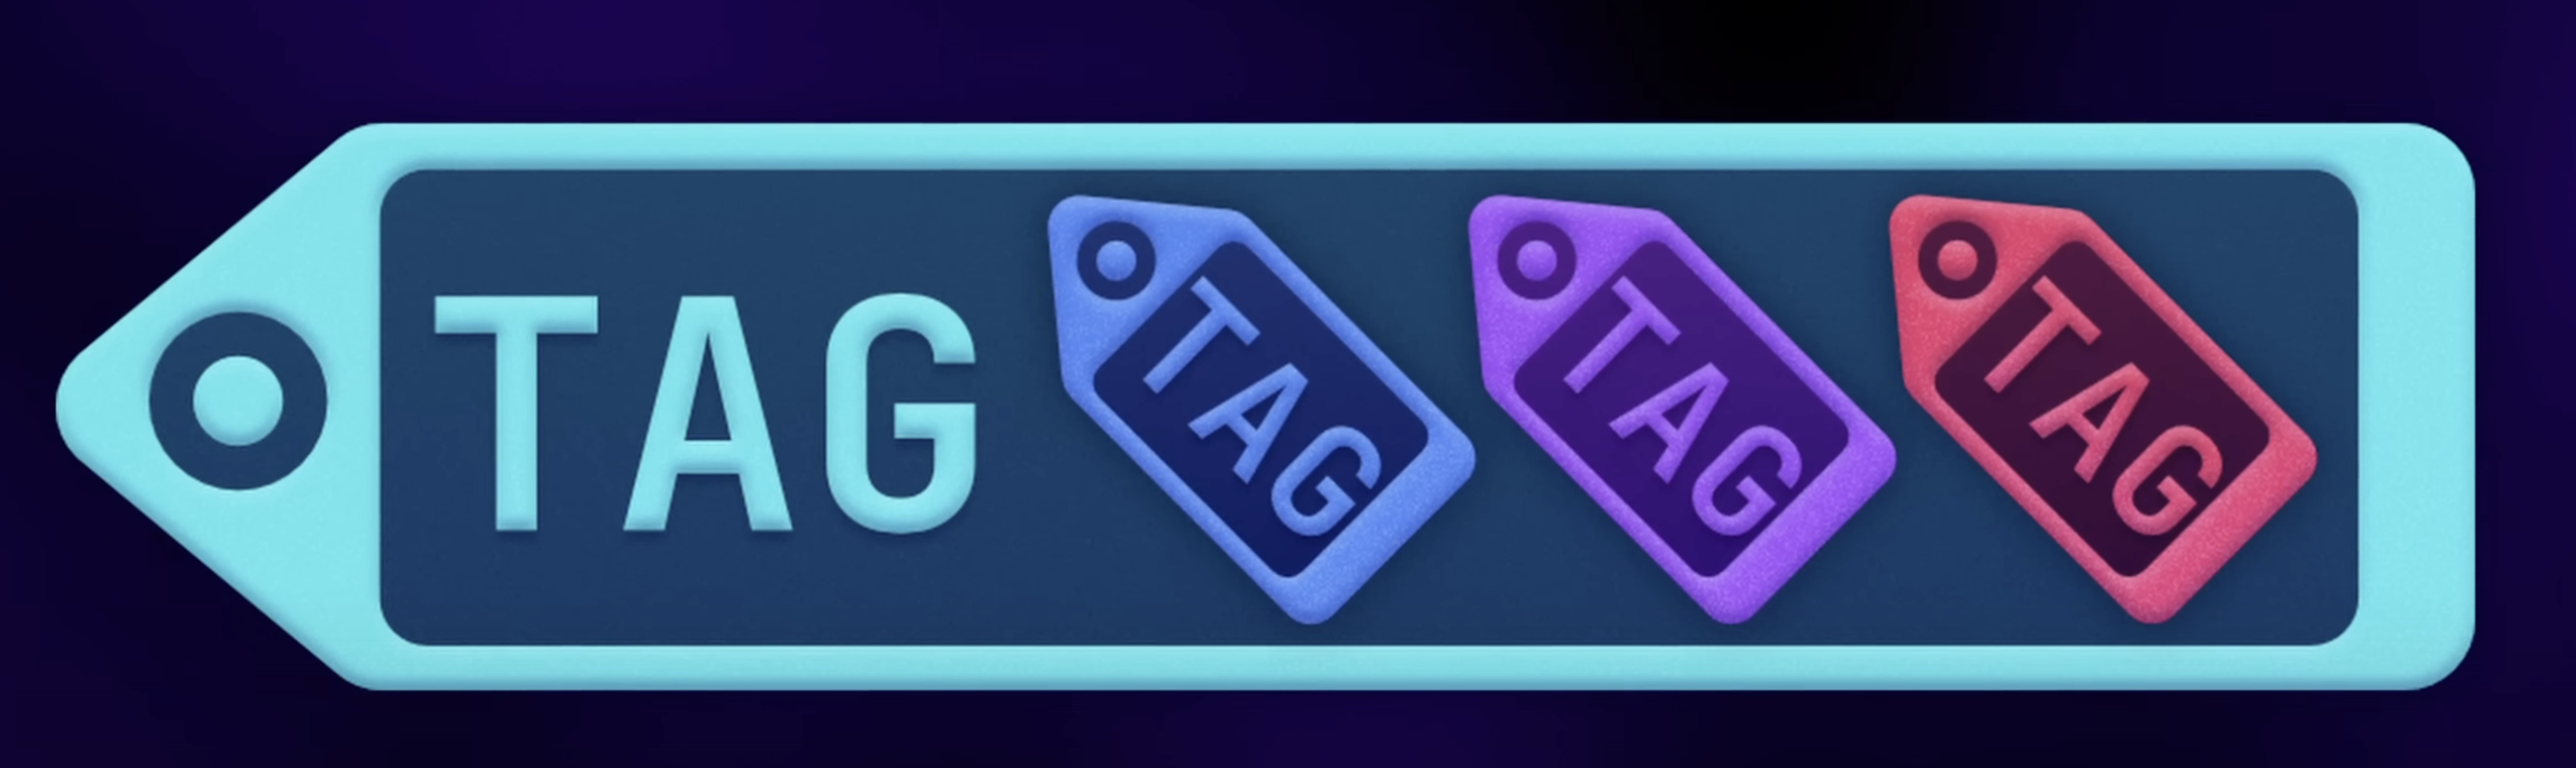
\includegraphics[width=0.8\textwidth]{Research/7_DataTagging/media/TagStudio.png}
    \caption{Illustration from the video showing nested tags}
\end{figure}
